\documentclass[a4paper, 12pt, oneside]{sastra}
\usepackage{amsmath}
\usepackage{times}
\usepackage{t1enc}
\usepackage[toc,page]{appendix}
\usepackage{graphicx}
\usepackage{epstopdf}
\usepackage{datetime}
\usepackage[driverfallback=dvipdfm]{hyperref}
%\usepackage[hypertex]{hyperref} % hyperlinks for references.
% easier math formulae, align, subequations \ldots

\begin{document}
	
	%\begin{document}
	
	%%%%%%%%%%%%%%%%%%%%%%%%%%%%%%%%%%%%%%%%%%%%%%%%%%%%%%%%%%%%%%%%%%%%%%
	%%%% OLD METHOD OF CREATING A FRONT PAGE %%%%%%%%%%%%%%
	\thispagestyle{empty}
	\begin{center}
		\Large{\textbf{Coordinated system for charging and discharging for different and various electric vehicles for energy management}}
	\end{center}
	\bigskip{}
	\bigskip{}
	\bigskip{}
	\begin{center}
		\textit{Report submitted to the SASTRA Deemed to be University\\ 
			as the requirement for the course\\
		}
		\bigskip{}
		\bigskip{}
		\large{\textbf{EEE300: MINI PROJECT}}
		\bigskip{}
		\bigskip{}
		\bigskip{}
		\bigskip{}
		\bigskip{}
		\bigskip{}
	\end{center}
	\begin{center}
		\textit{Submitted by}\\
	\end{center}
	\begin{center}
		\begin{singlespacing}
			\textbf{\Large{Mithra Vinda Reddy K}}
			
			\textbf{\large{(Reg. No.: 123005085)}}
			
			%\noalign{\smallskip}
			%\noalign{\smallskip}
			\textbf{\Large{Sarvesh babu R G}}
			
			\textbf{\large{(Reg. No.: 123005132)}}
			
			%\noalign{\smallskip}
			%\noalign{\smallskip}
			\textbf{\Large{Shwetha S}}
			
			\textbf{\large{(Reg. No.: 123005140)}}
		\end{singlespacing}
	\end{center}
	\bigskip{}
	
	\begin{center}
		\Large{\textbf{December 2022}}   %%%%%%%%%% if needed use capital 'L' or small 'l' for large
	\end{center}
	\bigskip{}
	\begin{center}
		\includegraphics[height=1.52in, width=5.65in]{SASTRA_Combined_Logo}
	\end{center}
	
	%\noalign{\smallskip}
	\begin{center}
		\large{\textbf{SCHOOL OF ELECTRICAL AND ELECTROINCS ENGINEERING}} %%%% contents in this line has to be 16
		{\textbf{THANJAVUR,TAMIL NADU, INDIA-613 401}}
	\end{center}
	
	%%%%%%%%%%%%%%%%%%%%%%%%%%%%%%%%%%%%%%%%%%%%%%%%%%%%%%%%%%%%%%%%%%%%%%
	
	%\title{PROJECT TITLE}
	
	%\author{BEECEE707: MINI PROJECT-II}
	
	%\date{MONTH 2021}
	
	%\department{ELECTRICAL \& ELECTRONICS ENGINEERING} %actually school name
	
	%\maketitle
	
	%%%%%%%%%%%%%%%%%%%%%%%%%%%%%%%%%%%%%%%%%%%%%%%%%%%%%%%%%%%%%%%%%%%%%%
	\newpage
	
	\pagenumbering{roman}
	\setcounter{page}{2}
	
	\certificate
	
	%\vspace*{0.5in}
	
	\begin{doublespace}
		\linespread{2}
		
		This is to certify that the report titled ``\textbf{Coordinated system for charging and discharging for different and various electric vehicles for energy management}'' submitted as a requirement for the course, {\textbf{EEE300: MINI PROJECT} for B. Tech. Electrical \& Electronics Engineering programme, is a bonafide record of the work done by \textbf{Ms.Mithra Vinda Reddy K ~~(Reg.No.123005085),~~Mr.Sarvesh Babu R G ~~(Reg.No.123005132),~~Ms.Shwetha S ~~(Reg.No.123005140)} during the academic year 2022-23, in the \textbf{School of Electrical and Electronics Engineering}, under my supervision.
			
	\end{doublespace}
	\vspace*{0.4in}
	
\noindent\textbf{Signature of Project Supervisor:}~	\\ %%%%%Remove this name while submission
\\
\textbf{Name with Affliation\hspace*{19mm}:~\textbf{Dr.~Narayanan K}~(SAP~/~EEE~/~SEEE)}	\\
\\
	\textbf{Date\hspace*{48.25mm}:}~31~/~03~/~2021\\%%%%%%% Add date after paranthesis while printing
	
	\vspace*{0.35in}
	
	\noindent Project \textit{Vivavoce} held on
	
	\vspace*{0.50in}
	\noindent \textbf{Examiner-I} \hspace*{120mm} \textbf{Examiner-II}
	
	%%%%%%%%%%%%%%%%%%%%%%%%%%%%%%%%%%%%%%%%%%%%%%%%%%%%%%%%%%%%%%%%%%%%%%
	
	\declaration
	
	%\vspace*{0.5in}
		
		\begin{doublespace}
		\linespread{2}
		
		I/We declare that the report titled ``\textbf{Coordinated system for charging and discharging for different and various electric vehicles for energy management}'' submitted by me/us is an original work done by me/us under the guidance of \textbf{Dr. Narayanan K, SAP, School of Electrical and Electronics Engineering, SASTRA Deemed to be University} during the academic year 2022-23, in the \textbf{School of Electrical and Electronics Engineering}. The work is original and wherever We have used materials from other sources, I/We have given due credit and cited them in the text of the report. This report has not formed the basis for the award of any degree, diploma, associate-ship, fellowship or other similar title to any candidate of any University.\\
		
	\end{doublespace}
	%\end{singlespacing}
	\noindent \textbf{Signature of the candidate(s)	:}	
	\\
	\\
	\\
	\\
	\\
	\noindent\textbf{Name of the candidate(s)\hspace{7mm}		: Mithra Vinda Reddy K}\\
	\hspace*{53mm}\textbf{: Sarvesh Babu R G}\\
	\hspace*{53mm}\textbf{: Shwetha S}\\
	\noindent\textbf{Date\hspace*{43.5mm}					:}~09~/~12~/~2022\\%%%%%%% Add date after paranthesis while printing
	
	%%%%%%%%%%%%%%%%%%%%%%%%%%%%%%%%%%%%%%%%%%%%%%%%%%%%%%%%%%%%%%%%%%%%%%
	% Acknowledgements
	\acknowledgements
	
	\hspace*{12pt} We express our gratitude to honourable \textbf{Dr.~S.~Vaidhyasubramaniam}, Vice Chancellor SASTRA University forcm the opportunity of pursuing our engineering in this esteemed in institution and carry out the project work.
	
	\par We thank \textbf{Dr.~R.~Chandramouli}, Registrar, SASTRA University for granting permission and extending the facilities in carrying out this project.
	
	\par We express our sincere thanks and gratitude to \textbf{Dr.~K.~Thenmozhi}, Dean, SEEE and \textbf{Dr.~K.~Vijayarekha}, Associate Dean, EEED/SEEE SASTRA Deemed to be University, for her support in the supporting the accomplishment of this work.
	
	\par We also render our sincere thanks to project coordinators, \textbf{Dr.~Karthikaikannan D}, SAP/EEE/SEEE and \textbf{Dr.~Venkatesh T}, AP-III/EEE/SEEE, SASTRA Deemed to be University for their involvement and encouragement during this project.
	
	\par We would like to thank our guide, \textbf{Dr.~Narayanan K}, SAP/EEE/SEEE, SASTRA Deemed to be University, for his guidance and support, that cumulated to his successful project. His emphasis on making learning an experience allowed us to learn while making mistakes and rectifying them to learn ,not only the scientific concepts behind power systems but also the process of analysing results.
	
	\par We would like to thank our friends who supported us. We would also like to thank the lab assistants for helping us with their practical expertise and for providing the necessary software tools.
	
	\par And finally, we would like to acknowledge the appreciation and support that our parents provided to ensure we faced minimal obstacles throughout the project.
	\pagebreak
	
	%%%%%%%%%%%%%%%%%%%%%%%%%%%%%%%%%%%%%%%%%%%%%%%%%%%%%%%%%%%%%%%%%%%%%%
	\abstract
	
	%\noindent KEYWORDS: \hspace*{0.5em} \parbox[t]{4.4in}{\LaTeX ; Thesis; Style files; Format.}
	
	\vspace*{24pt}
	
	\noindent A \LaTeX\ class along with a simple template thesis are provided here.  These can be used to easily write a thesis suitable for submission at IIT-Madras.  The class provides options to format PhD, MS, M.Tech.\ and B.Tech.\ thesis.  It also allows one to write a synopsis using the same class file.  Also provided is a BIB\TeX\ style file that formats all bibliography entries as per the IITM format.
	
	The formatting is as (as far as the author is aware) per the current institute guidelines.
	
	\noindent \textbf{Specific Contribution}
	\begin{itemize}
		\item It also allows one to write a synopsis using the same class file. It also allows one to write a synopsis using the same class file.
		\item It also allows one to write a synopsis using the same class file. It also allows one to write a synopsis using the same class file.
	\end{itemize}
	\noindent \textbf{Specific Learning}
	\begin{itemize}
		\item It also allows one to write a synopsis using the same class file. It also allows one to write a synopsis using the same class file.
		\item It also allows one to write a synopsis using the same class file. It also allows one to write a synopsis using the same class file.
	\end{itemize}
	
	\vspace*{24pt}
	
	\noindent \textbf{Signature of the Guide} \hspace*{66mm} \textbf{Student Reg. No:}121005206\\
		\\
	\\
	\\
	\noindent \textbf{Name of the Guide}:~Dr.~Name(Designation) \hspace*{31mm} \textbf{Name:}Your name
	\pagebreak
	
	%%%%%%%%%%%%%%%%%%%%%%%%%%%%%%%%%%%%%%%%%%%%%%%%%%%%%%%%%%%%%%%%%
	% for the second member
	\begin{center}
		\Large{{\textbf{ABSTRACT}}}
	\end{center}
	
	%\noindent KEYWORDS: \hspace*{0.5em} \parbox[t]{4.4in}{\LaTeX ; Thesis;Style files; Format.}
	
	\vspace*{24pt}
	
	\noindent A \LaTeX\ class along with a simple template thesis are provided here.  These can be used to easily write a thesis suitable for submission at IIT-Madras.  The class provides options to format PhD, MS, M.Tech.\ and B.Tech.\ thesis.  It also allows one to write a synopsis using the same class file.  Also provided is a BIB\TeX\ style file that formats all bibliography entries as per the IITM format.
	
	The formatting is as (as far as the author is aware) per the current institute guidelines.
	
	\noindent \textbf{Specific Contribution}
	\begin{itemize}
		\item It also allows one to write a synopsis using the same class file. It also allows one to write a synopsis using the same class file.
		\item It also allows one to write a synopsis using the same class file. It also allows one to write a synopsis using the same class file.
	\end{itemize}
	\noindent \textbf{Specific Learning}
	\begin{itemize}
		\item It also allows one to write a synopsis using the same class file. It also allows one to write a synopsis using the same class file.
		\item It also allows one to write a synopsis using the same class file. It also allows one to write a synopsis using the same class file.
	\end{itemize}
	
	\vspace*{24pt}
	
	\noindent \textbf{Signature of the Guide} \hspace*{66mm} \textbf{Student Reg. No:}121005206\\
		\\
	\\
	\\
\noindent \textbf{Name of the Guide}:~Dr.~Name(Designation) \hspace*{31mm} \textbf{Name:}Your name
\pagebreak
	%%%%%%%%%%%%%%%%%%%%%%%%%%%%%%%%%%%%%%%%%%%%%%%%%%%%%%%%%%%%%%%%%
	% for the third member
	
	\begin{center}
		\Large{{\textbf{ABSTRACT}}}
	\end{center}
	
	%\noindent KEYWORDS: \hspace*{0.5em} \parbox[t]{4.4in}{\LaTeX ; Thesis;Style files; Format.}
	
	\vspace*{24pt}
	
	\noindent A \LaTeX\ class along with a simple template thesis are provided here.  These can be used to easily write a thesis suitable for submission at IIT-Madras.  The class provides options to format PhD, MS, M.Tech.\ and B.Tech.\ thesis.  It also allows one to write a synopsis using the same class file.  Also provided is a BIB\TeX\ style file that formats all bibliography entries as per the IITM format.
	
	The formatting is as (as far as the author is aware) per the current institute guidelines.
	
	\noindent \textbf{Specific Contribution}
	\begin{itemize}
		\item It also allows one to write a synopsis using the same class file. It also allows one to write a synopsis using the same class file.
		\item It also allows one to write a synopsis using the same class file. It also allows one to write a synopsis using the same class file.
	\end{itemize}
	\noindent \textbf{Specific Learning}
	\begin{itemize}
		\item It also allows one to write a synopsis using the same class file. It also allows one to write a synopsis using the same class file.
		\item It also allows one to write a synopsis using the same class file. It also allows one to write a synopsis using the same class file.
	\end{itemize}
	
	\vspace*{24pt}
	
	\noindent \textbf{Signature of the Guide} \hspace*{66mm} \textbf{Student Reg. No:}121005206\\
		\\
	\\
	\\
\noindent \textbf{Name of the Guide}:~Dr.~Name(Designation) \hspace*{31mm} \textbf{Name:}Your name
\pagebreak
	
	
	
	%%%%%%%%%%%%%%%%%%%%%%%%%%%%%%%%%%%%%%%%%%%%%%%%%%%%%%%%%%%%%%%%%
	\begin{singlespace}
		\tableofcontents
		\thispagestyle{empty}
		
		
		\listoffigures
		\addcontentsline{toc}{chapter}{LIST OF FIGURES}
		\listoftables
		\addcontentsline{toc}{chapter}{LIST OF TABLES}
	\end{singlespace}
	
	
	%%%%%%%%%%%%%%%%%%%%%%%%%%%%%%%%%%%%%%%%%%%%%%%%%%%%%%%%%%%%%%%%%%%%%%
	\abbreviations
	
	\noindent 
	\begin{tabbing}
		xxxxxxxxxxx \= xxxxxxxxxxxxxxxxxxxxxxxxxxxxxxxxxxxxxxxxxxxxxxxx \kill
		\textbf{IITM}   \> Indian Institute of Technology, Madras \\
		\textbf{RTFM} \> Read the Fine Manual \\
	\end{tabbing}
	
	\pagebreak
	
	%%%%%%%%%%%%%%%%%%%%%%%%%%%%%%%%%%%%%%%%%%%%%%%%%%%%%%%%%%%%%%%%%%%%%%
	
	\chapter*{\centerline{NOTATIONS}}
	\addcontentsline{toc}{chapter}{NOTATIONS}
	
	\begin{singlespace}
		\begin{tabbing}
			xxxxxxxxxxx \= xxxxxxxxxxxxxxxxxxxxxxxxxxxxxxxxxxxxxxxxxxxxxxxx \kill
			\textbf{$r$}  \> Radius, $m$ \\
			\textbf{$\alpha$}  \> Angle of thesis in degrees \\
			\textbf{$\beta$}   \> Flight path in degrees \\
		\end{tabbing}
	\end{singlespace}
	
	\pagebreak
	\clearpage
	
	% The main text will follow from this point so set the page numbering
	% to arabic from here on.
	
	\pagenumbering{arabic}
	
	%%%%%%%%%%%%%%%%%%%%%%%%%%%%%%%%%%%%%%%%%%%%%%%%%%
	%%% More chapters can be added if necessary
		\chapter{INTRODUCTION}
	\label{chap:intro}
	
	\section{Electric Vehicle}
	
	With the increase in Pollution , fuel demand, global warming and many other socio-economic issues ,one could say Electric Vehicles will be the future means of transport.
	
	
	\section{*****}
	\section{*****}
	\section{*****}
	\section{*****}
	\section{Motivation}
	This document provides a simple template of how the provided
	\verb+iitmdiss.cls+ \LaTeX\ class is to be used.  Also provided are
	several useful tips to do various things that might be of use when you
	write your thesis.
	
	Before reading any further please note that you are strongly advised
	against changing any of the formatting options used in the class
	provided in this directory, unless you are absolutely sure that it
	does not violate the IITM formatting guidelines.  \emph{Please do not
		change the margins or the spacing.}  If you do change the formatting
	you are on your own (don't blame me if you need to reprint your entire
	thesis).  In the case that you do change the formatting despite these
	warnings, the least I ask is that you do not redistribute your style
	files to your friends (or enemies).
	
	It is also a good idea to take a quick look at the formatting
	guidelines.  Your office or advisor should have a copy.  If they
	don't, pester them, they really should have the formatting guidelines
	readily available somewhere.
	
	To compile your sources run the following from the command line:
	\begin{verbatim}
	% latex thesis.tex
	% bibtex thesis
	% latex thesis.tex
	% latex thesis.tex
	\end{verbatim}
	Modify this suitably for your sources.
	
	To generate PDF's with the links from the \verb+hyperref+ package use
	the following command:
	\begin{verbatim}
	% dvipdfm -o thesis.pdf thesis.dvi
	\end{verbatim}
	
	\section{Package Options}
	
	Use this thesis as a basic template to format your thesis.  The
	\verb+iitmdiss+ class can be used by simply using something like this:
	\begin{verbatim}
	\documentclass[PhD]{iitmdiss}  
	\end{verbatim}
	
	To change the title page for different degrees just change the option
	from \verb+PhD+ to one of \verb+MS+, \verb+MTech+ or \verb+BTech+.
	The dual degree pages are not supported yet but should be quite easy
	to add.  The title page formatting really depends on how large or
	small your thesis title is.  Consequently it might require some hand
	tuning.  Edit your version of \verb+iitmdiss.cls+ suitably to do this.
	I recommend that this be done once your title is final.
	
	To write a synopsis simply use the \verb+synopsis.tex+ file as a
	simple template.  The synopsis option turns this on and can be used as
	shown below.
	\begin{verbatim}
	\documentclass[PhD,synopsis]{iitmdiss}                                
	\end{verbatim}
	
	Once again the title page may require some small amount of fine
	tuning.  This is again easily done by editing the class file.
	
	This sample file uses the \verb+hyperref+ package that makes all
	labels and references clickable in both the generated DVI and PDF
	files.  These are very useful when reading the document online and do
	not affect the output when the files are printed.
	
	
	\section{Example Figures and tables}
	
	Fig.~\ref{fig:iitm} shows a simple figure for illustration along with
	a long caption.  The formatting of the caption text is automatically
	single spaced and indented.  Table~\ref{tab:sample} shows a sample
	table with the caption placed correctly.  The caption for this should
	always be placed before the table as shown in the example.
	
	
	\begin{figure}[htpb]
		\begin{center}
			\resizebox{50mm}{!} {\includegraphics *{iitm.eps}}
			\resizebox{50mm}{!} {\includegraphics *{iitm.eps}}
			\caption {Two IITM logos in a row.  This is also an
				illustration of a very long figure caption that wraps around two
				two lines.  Notice that the caption is single-spaced.}
			\label{fig:iitm}
		\end{center}
	\end{figure}
	
	\begin{table}[htbp]
		\caption{A sample table with a table caption placed
			appropriately. This caption is also very long and is
			single-spaced.  Also notice how the text is aligned.}
		\begin{center}
			\begin{tabular}[c]{|c|r|} \hline
				$x$ & $x^2$ \\ \hline
				1  &  1   \\
				2  &  4  \\
				3  &  9  \\
				4  &  16  \\
				5  &  25  \\
				6  &  36  \\
				7  &  49  \\
				8  &  64  \\ \hline
			\end{tabular}
			\label{tab:sample}
		\end{center}
	\end{table}
	
	\section{Bibliography with BIB\TeX}
	
	I strongly recommend that you use BIB\TeX\ to automatically generate
	your bibliography.  It makes managing your references much easier.  It
	is an excellent way to organize your references and reuse them.  You
	can use one set of entries for your references and cite them in your
	thesis, papers and reports.  If you haven't used it anytime before
	please invest some time learning how to use it.  
	
	I've included a simple example BIB\TeX\ file along in this directory
	called \verb+refs.bib+.  The \verb+iitmdiss.cls+ class package which
	is used in this thesis and for the synopsis uses the \verb+natbib+
	package to format the references along with a customized bibliography
	style provided as the \verb+iitm.bst+ file in the directory containing
	\verb+thesis.tex+.  Documentation for the \verb+natbib+ package should
	be available in your distribution of \LaTeX.  Basically, to cite the
	author along with the author name and year use \verb+\cite{key}+ where
	\verb+key+ is the citation key for your bibliography entry.  You can
	also use \verb+\citet{key}+ to get the same effect.  To make the
	citation without the author name in the main text but inside the
	parenthesis use \verb+\citep{key}+.  The following paragraph shows how
	citations can be used in text effectively.
	
	More information on BIB\TeX\ is available in the book by
	\cite{lamport:86}.  There are many
	references~\cite{lamport:86,prabhu:xx} that explain how to use
	BIB\TeX.  Read the \verb+natbib+ package documentation for more
	details on how to cite things differently.
	
	Here are other references for example.  \cite{viz:mayavi} presents a
	Python based visualization system called MayaVi in a conference paper.
	\cite{pan:pr:flat-fst} illustrates a journal article with multiple
	authors.  Python~\cite{py:python} is a programming language and is
	cited here to show how to cite something that is best identified with
	a URL.
	
	\section{Other useful \LaTeX\ packages}
	
	The following packages might be useful when writing your thesis.
	
	\begin{itemize}  
		\item It is very useful to include line numbers in your document.
		That way, it is very easy for people to suggest corrections to your
		text.  I recommend the use of the \texttt{lineno} package for this
		purpose.  This is not a standard package but can be obtained on the
		internet.  The directory containing this file should contain a
		lineno directory that includes the package along with documentation
		for it.
		
		\item The \texttt{listings} package should be available with your
		distribution of \LaTeX.  This package is very useful when one needs
		to list source code or pseudo-code.
		
		\item For special figure captions the \texttt{ccaption} package may be
		useful.  This is specially useful if one has a figure that spans
		more than two pages and you need to use the same figure number.
		
		\item The notation page can be entered manually or automatically
		generated using the \texttt{nomencl} package.
		
	\end{itemize}
	
	More details on how to use these specific packages are available along
	with the documentation of the respective packages.
	
	\chapter{LITERATURE SURVEY}
	\label{chap:obj}
	
	The objectives of this project are:
	\begin{itemize}
		\item 
		\item 
		\item
	\end{itemize}
	
		\chapter{METHODOLOGY}
	\label{chap:work}
	
	\section{Vehicle Classification}
	
	 Electric vehicles have been classified primarily into four major categories as shown in Figure~\ref{fig:classification} 
	 	
			\begin{figure}[h]
				\centering
				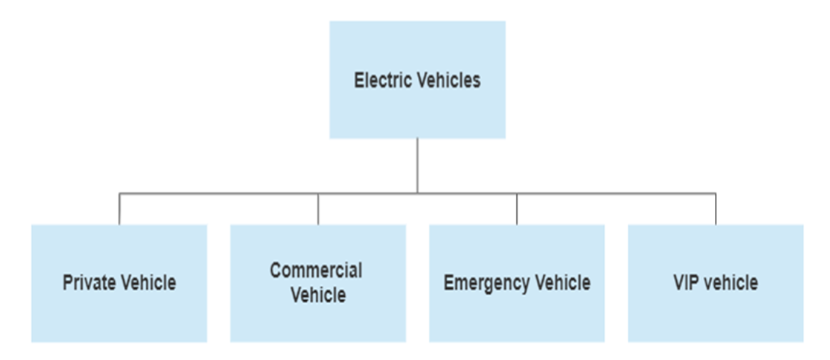
\includegraphics[width=0.7\linewidth]{classification}
				\caption{Vehicle Classification}
				\label{fig:classification}
			\end{figure}
		
	The above classification is made by comparing the battery capacity of the vehicles from the data \cite{evdata} taken with the battery capacity of the similar kind of vehicles in the market.

	\par {Private vehicles are further classified into E-bikes and E-cars with average battery capacity of 400Wh to 500 Wh and 40 kWh to 100 Kwh respectively. Commercial vehicles are classified into E-Truck and E-Bus with an average battery capacity of 100 KWh and 60 to 548 KWh respectively. Emergency vehicles have a battery capacity of around 105 KWh and VIP vehicles have around 90 KWh to 200 KWh.
	}
	
	\section{Travel Pattern Establishment}
	
	Travel pattern for three main vehicle subcategories of the above mentioned vehicle categories namely E-car, E-Truck and E-Bus are now taken and travel patterns of the same have been established by using the Battery capacity, Time taken to full charge, Time period of the vehicle when it is connected to the grid , charging rate and discharging rate.
	
	\section{Charging/Discharging Pattern}
	
	\section{Proposed Algorithm}
		\begin{figure}
			\centering
			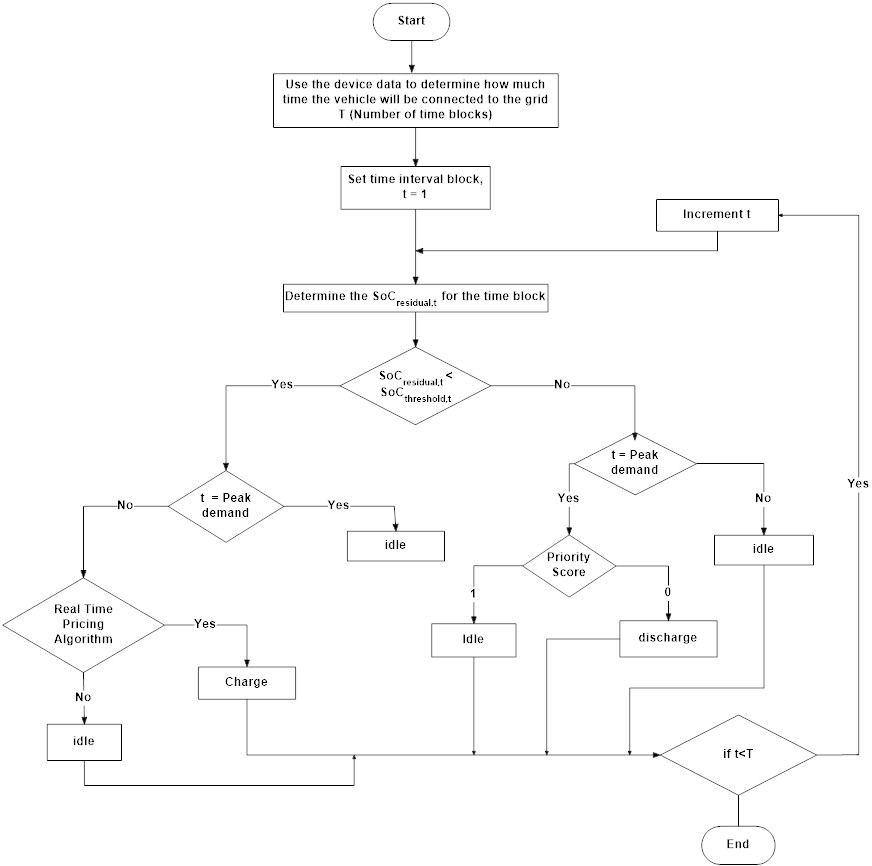
\includegraphics[width=1\linewidth]{Ev_flowchart}
			\caption{Proposed Algorithm for determining Charging/Discharging Pattern}
			\label{fig:evflowchart}
		\end{figure}
		
	
	
	
	
	\chapter{RESULTS \& DISCUSSION}
	\label{chap:results}
	
	\section{Tabulations}
	
	
	\begin{table}[h]
		\centering
		\begin{tabular}{|cl|ll|ll|ll|}
			\hline
			\multicolumn{2}{|c|}{\multirow{2}{*}{\textbf{SCENARIO}}} & \multicolumn{2}{c|}{\textbf{Case 1 - (00:00)}}                                                                                                                                                                                   & \multicolumn{2}{c|}{\textbf{Case 2 - (00:20)}}                                                                                                                                                                                   & \multicolumn{2}{c|}{\textbf{Case 3 - (00:40)}}                                                                                                                                                                                   \\ \cline{3-8} 
			\multicolumn{2}{|c|}{}                                   & \multicolumn{1}{c|}{\textbf{\begin{tabular}[c]{@{}c@{}}Power Loss \\ when Ev in \\ Bus 2 (W)\end{tabular}}} & \multicolumn{1}{c|}{\textbf{\begin{tabular}[c]{@{}c@{}}Power Loss \\ when Ev in \\ Bus 18 (W)\end{tabular}}} & \multicolumn{1}{c|}{\textbf{\begin{tabular}[c]{@{}c@{}}Power Loss \\ when Ev in \\ Bus 2 (W)\end{tabular}}} & \multicolumn{1}{c|}{\textbf{\begin{tabular}[c]{@{}c@{}}Power Loss \\ when Ev in \\ Bus 18 (W)\end{tabular}}} & \multicolumn{1}{c|}{\textbf{\begin{tabular}[c]{@{}c@{}}Power Loss \\ when Ev in \\ Bus 2 (W)\end{tabular}}} & \multicolumn{1}{c|}{\textbf{\begin{tabular}[c]{@{}c@{}}Power Loss \\ when Ev in \\ Bus 18 (W)\end{tabular}}} \\ \hline
			\multicolumn{2}{|c|}{\textbf{SCENARIO-1}}                & \multicolumn{1}{l|}{204.1038}                                                                                  & 253.746                                                                                                         & \multicolumn{1}{l|}{65.7725}                                                                                   & 78.4603                                                                                                         & \multicolumn{1}{l|}{204.1038}                                                                                  & 253.746                                                                                                         \\ \hline
			\multicolumn{2}{|c|}{\textbf{SCENARIO-2}}                & \multicolumn{1}{l|}{189.8325}                                                                                  & 236.9117                                                                                                        & \multicolumn{1}{l|}{178.9671}                                                                                  & 222.4681                                                                                                        & \multicolumn{1}{l|}{189.8325}                                                                                  & 236.9117                                                                                                        \\ \hline
		\end{tabular}
		\caption{Power Loss when Ev connected in different busses in 33 bus system for two load profile scenarios}
	\end{table}


		\begin{table}[h]
			\centering
			\begin{tabular}{|l|l|l|}
				\hline
				\textbf{Scenario}         & \textbf{Best price} & \textbf{Hour} \\ \hline
				\textbf{Case 1 - (00:00)} & - \$1.71            & 12:00         \\ \hline
				\textbf{Case 2 - (00:20)} & - \$2.0988          & 01:20         \\ \hline
				\textbf{Case 3 - (00:40)} & - \$1.584           & 01:40         \\ \hline
			\end{tabular}
			\caption{Best pricing for Car during various connection time}
		\end{table}

		\begin{table}[h]
			\centering
			\begin{tabular}{|l|l|l|}
				\hline
				\textbf{Scenario}         & \textbf{Best price} & \textbf{Hour} \\ \hline
				\textbf{Case 1 - (00:00)}  & - \$2.579304 & 05:00         \\ \hline
				\textbf{Case 2 - (00:20)} & - \$1.003062667 & 04:20         \\ \hline
				\textbf{Case 3 - (00:40)} & - \$2.110840667 & 04:40         \\ \hline
			\end{tabular}
			\caption{Best pricing for Truck during various connection time}
		\end{table}



		\begin{table}[h]
			\centering
			\begin{tabular}{|l|l|l|}
				\hline
				\textbf{Scenario}         & \textbf{Best price} & \textbf{Hour} \\ \hline
				\textbf{Case 1 - (00:00)}  & - \$0.4791666667   & 12:00         \\ \hline
				\textbf{Case 2 - (00:20)} & - \$1.25         & 20:20         \\ \hline
				\textbf{Case 3 - (00:40)} & - \$0.6958333333 & 11:40         \\ \hline
			\end{tabular}
			\caption{Best pricing for Bus during various connection time}
		\end{table}
	
	\begin{table}[h]
		\centering
		\begin{tabular}{|ll|ll|ll|ll|}
			\hline
			\multicolumn{2}{|l|}{\textbf{SCENARIO}} & \multicolumn{2}{l|}{\textbf{HOURLY}} & \multicolumn{2}{l|}{\textbf{20MINS}} & \multicolumn{2}{l|}{\textbf{40 MINS}} \\ \hline
			\multicolumn{2}{|l|}{SCENARIO 1}        & \multicolumn{2}{l|}{13th}            & \multicolumn{2}{l|}{6th}             & \multicolumn{2}{l|}{13th}             \\ \hline
			\multicolumn{2}{|l|}{SCENARIO 2}        & \multicolumn{2}{l|}{19th}            & \multicolumn{2}{l|}{6th}             & \multicolumn{2}{l|}{19th}             \\ \hline
		\end{tabular}
		\caption{Hour at which the EV Load is maximum }
	\end{table}
		
	
	
	\section{Voltage Magnitude Graphs for Different Scenarios}
	
		\includegraphics[width=0.55\linewidth]{"sc 1 (00_00)"}
		\includegraphics[width=0.55\linewidth]{"sc 1 (00_20)"}
		\includegraphics[width=0.55\linewidth]{"sc 1 (00_40)"}
		\includegraphics[width=0.55\linewidth]{"sc 2 (00_00)"}
		\includegraphics[width=0.55\linewidth]{"sc 2 (00_20)"}
		\includegraphics[width=0.55\linewidth]{"sc 2 (00_40)"}
	
	\section{*****}
	
		\chapter{CONCLUSIONS AND FURTHER WORK}
	\label{chap:conclusion}
	
		\noindent A \LaTeX\ class along with a simple template thesis are provided here.  These can be used to easily write a thesis suitable for submission at IIT-Madras.  The class provides options to format PhD, MS, M.Tech.\ and B.Tech.\ thesis.  It also allows one to write a synopsis using the same class file.  Also provided is a BIB\TeX\ style file that formats all bibliography entries as per the IITM format.
	
	
	
	\vspace*{24pt}
	
	\noindent \textbf{Signature of the Guide} \hspace*{70mm} \textbf{Student Reg. No:}121005206\\
		\\
	\\
	\\
\noindent \textbf{Name of the Guide}:~Dr.~Name(Designation) \hspace*{35mm} \textbf{Name:}Your name
\pagebreak
	\pagebreak
	
	%%%%%%%%%%%%%%%%%%%%%%%%%%%%%%%%%%%%%%%%%%%%%%%%%%%%%%%%%%%%%%%%%
	% for the second member

	\begin{center}
		\Large{{\textbf{CONCLUSIONS}}}
	\end{center}
	
		\noindent A \LaTeX\ class along with a simple template thesis are provided here.  These can be used to easily write a thesis suitable for submission at IIT-Madras.  The class provides options to format PhD, MS, M.Tech.\ and B.Tech.\ thesis.  It also allows one to write a synopsis using the same class file.  Also provided is a BIB\TeX\ style file that formats all bibliography entries as per the IITM format.
	
	\vspace*{24pt}
	
	\noindent \textbf{Signature of the Guide} \hspace*{70mm} \textbf{Student Reg. No:}121005206\\
		\\
	\\
	\\
\noindent \textbf{Name of the Guide}:~Dr.~Name(Designation) \hspace*{35mm} \textbf{Name:}Your name
\pagebreak
	\pagebreak
	
	
	%%%%%%%%%%%%%%%%%%%%%%%%%%%%%%%%%%%%%%%%%%%%%%%%%%%%%%%%%%%%
	% for the third member
	\begin{center}
		\Large{{\textbf{CONCLUSIONS}}}
	\end{center}
	
		\noindent A \LaTeX\ class along with a simple template thesis are provided here.  These can be used to easily write a thesis suitable for submission at IIT-Madras.  The class provides options to format PhD, MS, M.Tech.\ and B.Tech.\ thesis.  It also allows one to write a synopsis using the same class file.  Also provided is a BIB\TeX\ style file that formats all bibliography entries as per the IITM format.
	
	\vspace*{24pt}
	
		\noindent \textbf{Signature of the Guide} \hspace*{70mm} \textbf{Student Reg. No:}121005206\\
			\\
		\\
		\\
	\noindent \textbf{Name of the Guide}:~Dr.~Name(Designation) \hspace*{35mm} \textbf{Name:}Your name
	\pagebreak
	\pagebreak
	
	
	%%%%%%%%%%%%%%%%%%%%%%%%%%%%%%%%%%%%%%%%%%%%%%%%%%%%%%%%%%%%
	%%%%%%%%%%%%%%%%%%%%%%%%%%%%%%%%%%%%%%%%%%%%%%%%%%%%%%%%%%%%%%%%%

% Bibliography.
\addcontentsline{toc}{chapter}{REFERENCES}
%\chapter{REFERENCES}
%\label{chap:refs}
%\bibliographystyle{plain}
%\bibliography{mybib}
\begin{singlespace}
%\section{REFERENCES}
%\bibliography{MyCollection}.
\bibliography{refs}
\end{singlespace}

%%%%%%%%%%%%%%%%%%%%%%%%%%%%%%%%%%%%%%%%%%%%%%%%%%%%%%%%%%%%

\listofpapers %%%% If there is no publications remove this section

\begin{enumerate}  
	\item Authors....  \newblock
	Title...
	\newblock {\em Journal}, Volume,
	Page, (year).
\end{enumerate} 

%%%%%%%%%%%%%%%%%%%%%%%%%%%%%%%%%%%%%%%%%%%%%%%%%%%%%%%%%%%%
% Appendices.

\appendix
%\addcontentsline{toc}{chapter}{APPENDICES}
%\begin{appendices}
%
\chapter{FIRST SET DATA}
%
%%Just put in text as you would into any chapter with sections and
%%whatnot.  Thats the end of it.
%
%%%%%%%%%%%%%%%%%%%%%%%%%%%%%%%%%%%%%%%%%%%%%%%%%%%%%%%%%%%%%
%
%
\chapter{SECOND SET DATA}
%
%%Just put in text as you would into any chapter with sections and
%%whatnot.  Thats the end of it.
%
%%%%%%%%%%%%%%%%%%%%%%%%%%%%%%%%%%%%%%%%%%%%%%%%%%%%%%%%%%%%%
%
%
%\chapter{THIRD SET DATA}
%
%%Just put in text as you would into any chapter with sections and
%%whatnot.  Thats the end of it.
%\end{appendices}


%%%%%%%%%%%%%%%%%%%%%%%%%%%%%%%%%%%%%%%%%%%%%%%%%%%%%%%%%%%%


\plagarism
\end{document}
